\documentclass[aspectratio=169]{beamer}
\DeclareOptionBeamer{shadow}[true]{\def\beamer@themerounded@shadow{#1}}
\ExecuteOptionsBeamer{shadow=true}
\ProcessOptionsBeamer

% favorite themes: AnnArbor, Frankfurt, Madrid, Luebeck
\mode<presentation>{\usetheme{Luebeck}}

% Color modification
% primary
\definecolor{UAblue}{RGB}{12, 35, 75}
\definecolor{UAdarkblue}{RGB}{0, 25, 74}
\definecolor{UAred}{RGB}{171, 5, 32}
\definecolor{UAdarkred}{RGB}{143, 17, 36}

% secondary
\definecolor{cactus}{RGB}{92, 135, 39}
\definecolor{sky}{RGB}{132, 210, 226}
\definecolor{river}{RGB}{7, 104, 115}
\definecolor{sand}{RGB}{241, 158, 31}
\definecolor{mesa}{RGB}{185, 85, 39}
\definecolor{brick}{RGB}{74, 48, 39}

% neutral palette
\definecolor{lightcactus}{RGB}{207, 224, 216}
\definecolor{lightsky}{RGB}{200, 217, 216}
\definecolor{lightriver}{RGB}{182, 190, 193}
\definecolor{lightsand}{RGB}{252, 225, 182}
\definecolor{lightmesa}{RGB}{250, 231, 216}
\definecolor{lightbrick}{RGB}{230, 227, 217}

\setbeamercolor{section in toc}{fg=UAdarkred,bg=white}
\setbeamercolor{subsection in toc}{fg=UAdarkred,bg=white}
\setbeamercolor*{palette primary}{fg=white,bg=UAblue}
\setbeamercolor*{palette secondary}{fg=UAdarkblue,bg=lightriver}
\setbeamercolor*{palette tertiary}{fg=white,bg=UAred}
\setbeamercolor*{palette quaternary}{fg=white,bg=UAred}
\setbeamercolor{title}{fg=white,bg=UAblue}
\setbeamercolor{titlelike}{fg=white,bg=UAblue}
\setbeamercolor{frametitle}{bg=lightriver,fg=UAdarkblue}
\setbeamercolor{frametitle right}{fg=white}
\setbeamercolor*{separation line}{fg=UAblue}
\setbeamercolor*{fine separation line}{fg=UAblue}

% block colors
\setbeamercolor{block title}{fg=white,bg=UAblue}
\setbeamercolor{block title alerted}{fg=white,bg=UAdarkred}
\setbeamercolor{block title example}{fg=white,bg=cactus}

% make some nice edges and shadow
\setbeamertemplate{blocks}[rounded][shadow=\beamer@themerounded@shadow]
\setbeamertemplate{items}[circle]
\setbeamercolor{item}{fg=UAblue}
\setbeamertemplate{sections/subsections in toc}[circle]
\setbeamertemplate{title page}[default][colsep=-4bp,rounded=true,shadow=\beamer@themerounded@shadow]
\setbeamertemplate{part
  page}[default][colsep=-4bp,rounded=true,shadow=\beamer@themerounded@shadow]

% logo, depending on title, may move this around to fit on page
% properly with vspace and hspace
\titlegraphic{\vspace{+0.5cm} 
\includegraphics[height=1cm]{ua_stack_rgb_0.pdf}}

% hyperlinks
\hypersetup{colorlinks,linkcolor=,urlcolor=river}

%% packages
\usepackage{amsmath}
%\usepackage{listings}
%\usepackage{relsize}
%\usepackage{multimedia}
%\usepackage{lipsum}
\usepackage[caption=false,font=footnotesize]{subfig}
%\usepackage[ampersand]{easylist}
\usepackage{natbib}
\usepackage{bibentry}


\title[Dissertation Proposal]{DESIGN AND USE OF AN IRRADIANCE
  MONITORING NETWORK FOR SHORT-TERM IRRADIANCE FORECASTING}
\author[Lorenzo]{Antonio T. Lorenzo}
\institute{University of Arizona}
\date{Feb. 22, 2017}
\subject{Dissertation Proposal}

% \AtBeginSection[]{
% \begin{frame}<beamer>
%   \frametitle{Outline}
%   \tableofcontents[currentsection]
% \end{frame}
% \addtocounter{framenumber}{-1} % remove for proper page numbers on
%                                % intermediate outline pages
% }

\begin{document}
\begin{frame}
  \titlepage
\end{frame}


\section{Importance of Irradiance Forecasts}
\label{sec:intro}

\begin{frame}{Operational Forecasting}
\begin{columns}
\begin{column}{0.5\textwidth}
\begin{figure}[h]
\centering
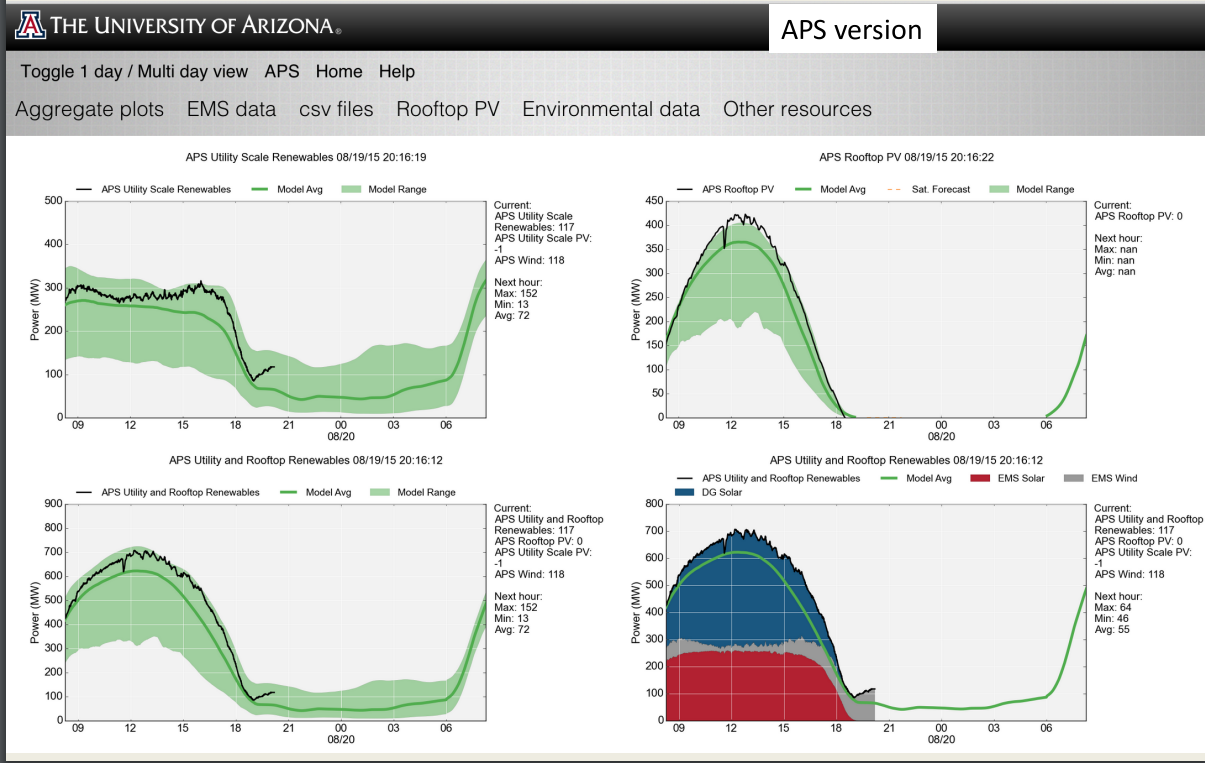
\includegraphics[width=\textwidth]{figs/website.png}
\end{figure}
\end{column}
\begin{column}{0.5\textwidth}
\begin{figure}[h]
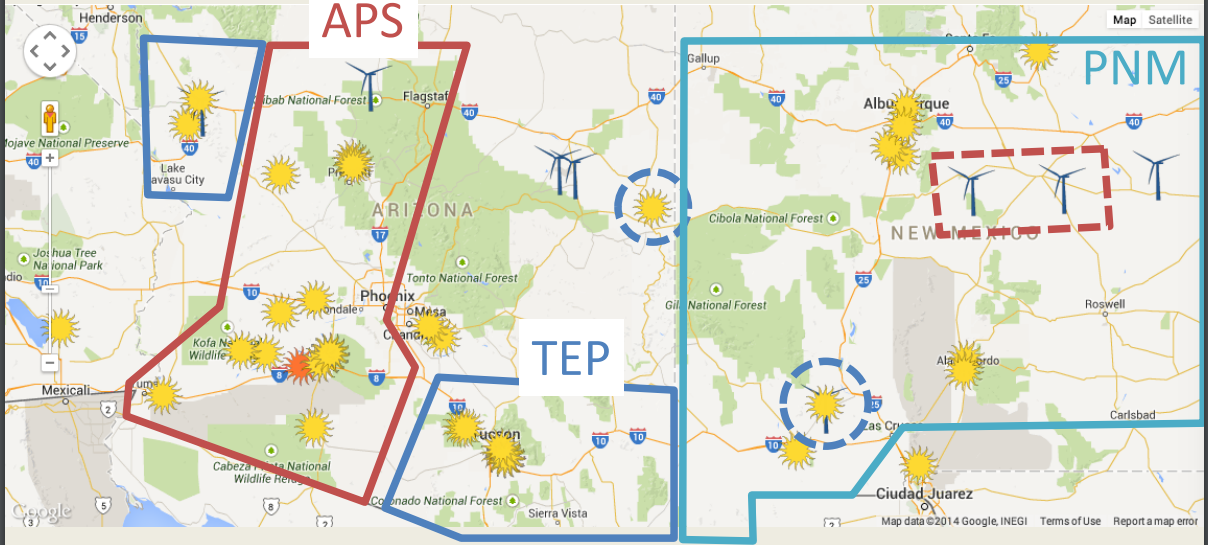
\includegraphics[width=\textwidth]{figs/utilities.png}
\end{figure}
\end{column}
\end{columns}
\end{frame}


\begin{frame}{Theoretical Errors}
\begin{figure}[h]
  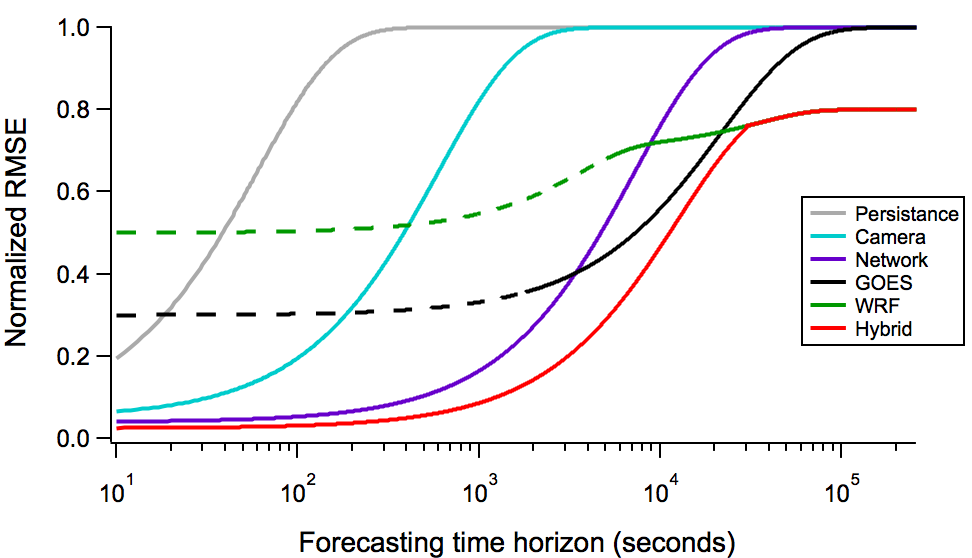
\includegraphics[height=.7\textheight]{figs/original_bullshit.png}
  \caption{Theoretical forecast errors circa 2013.}
\end{figure}
\end{frame}

\begin{frame}{Actual Errors}
\begin{figure}[h]
  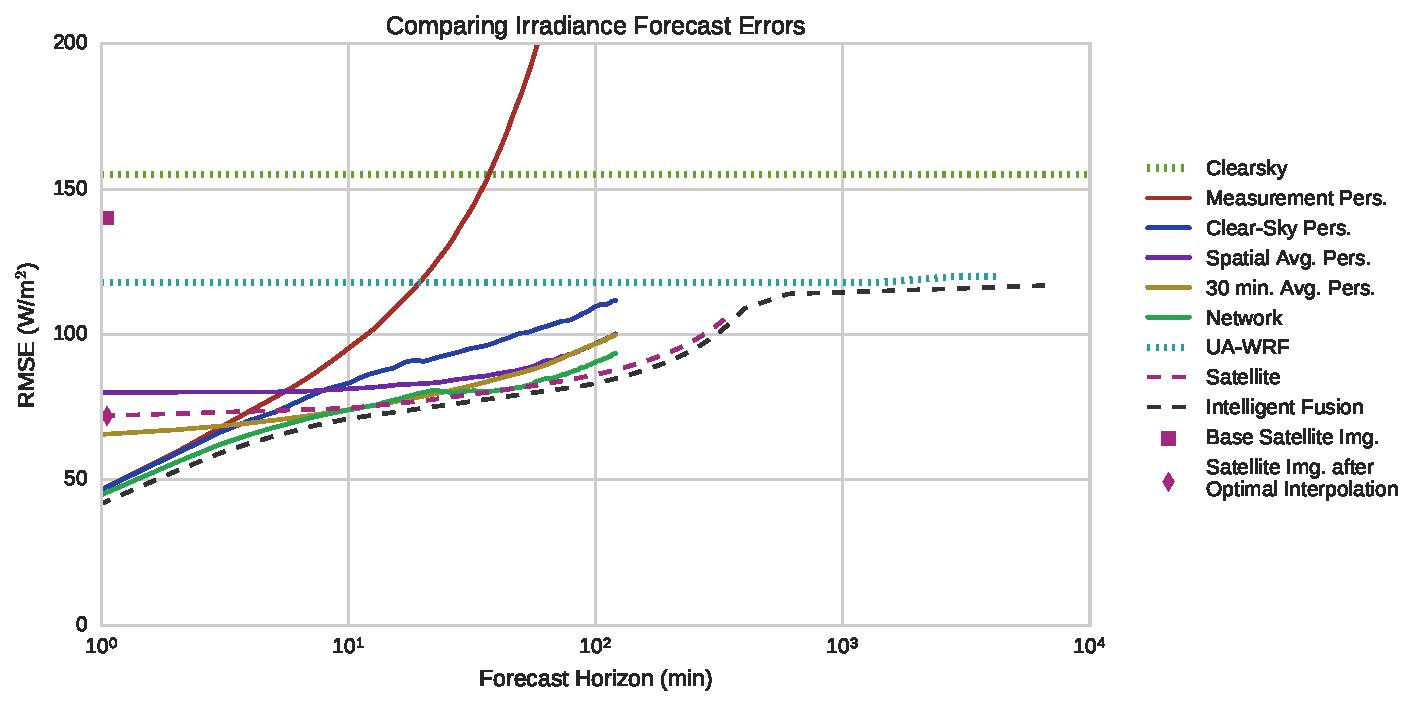
\includegraphics[width=.7\textwidth]{../dissertation/figs/timehorizon.pdf}
  \caption{Actual forecast errors as a result of my research. Solid lines
    and points are those studied in this dissertation. Dashed are preliminary
    or theoretical estimates.}
\end{figure}
\end{frame}


\begin{frame}{Outline}
  \tableofcontents
\end{frame}

\section{Design of Irradiance Monitoring Network}
\begin{frame}{Irradiance Network}
\begin{columns}
\begin{column}{0.3\textwidth}
\begin{figure}[h]
\centering
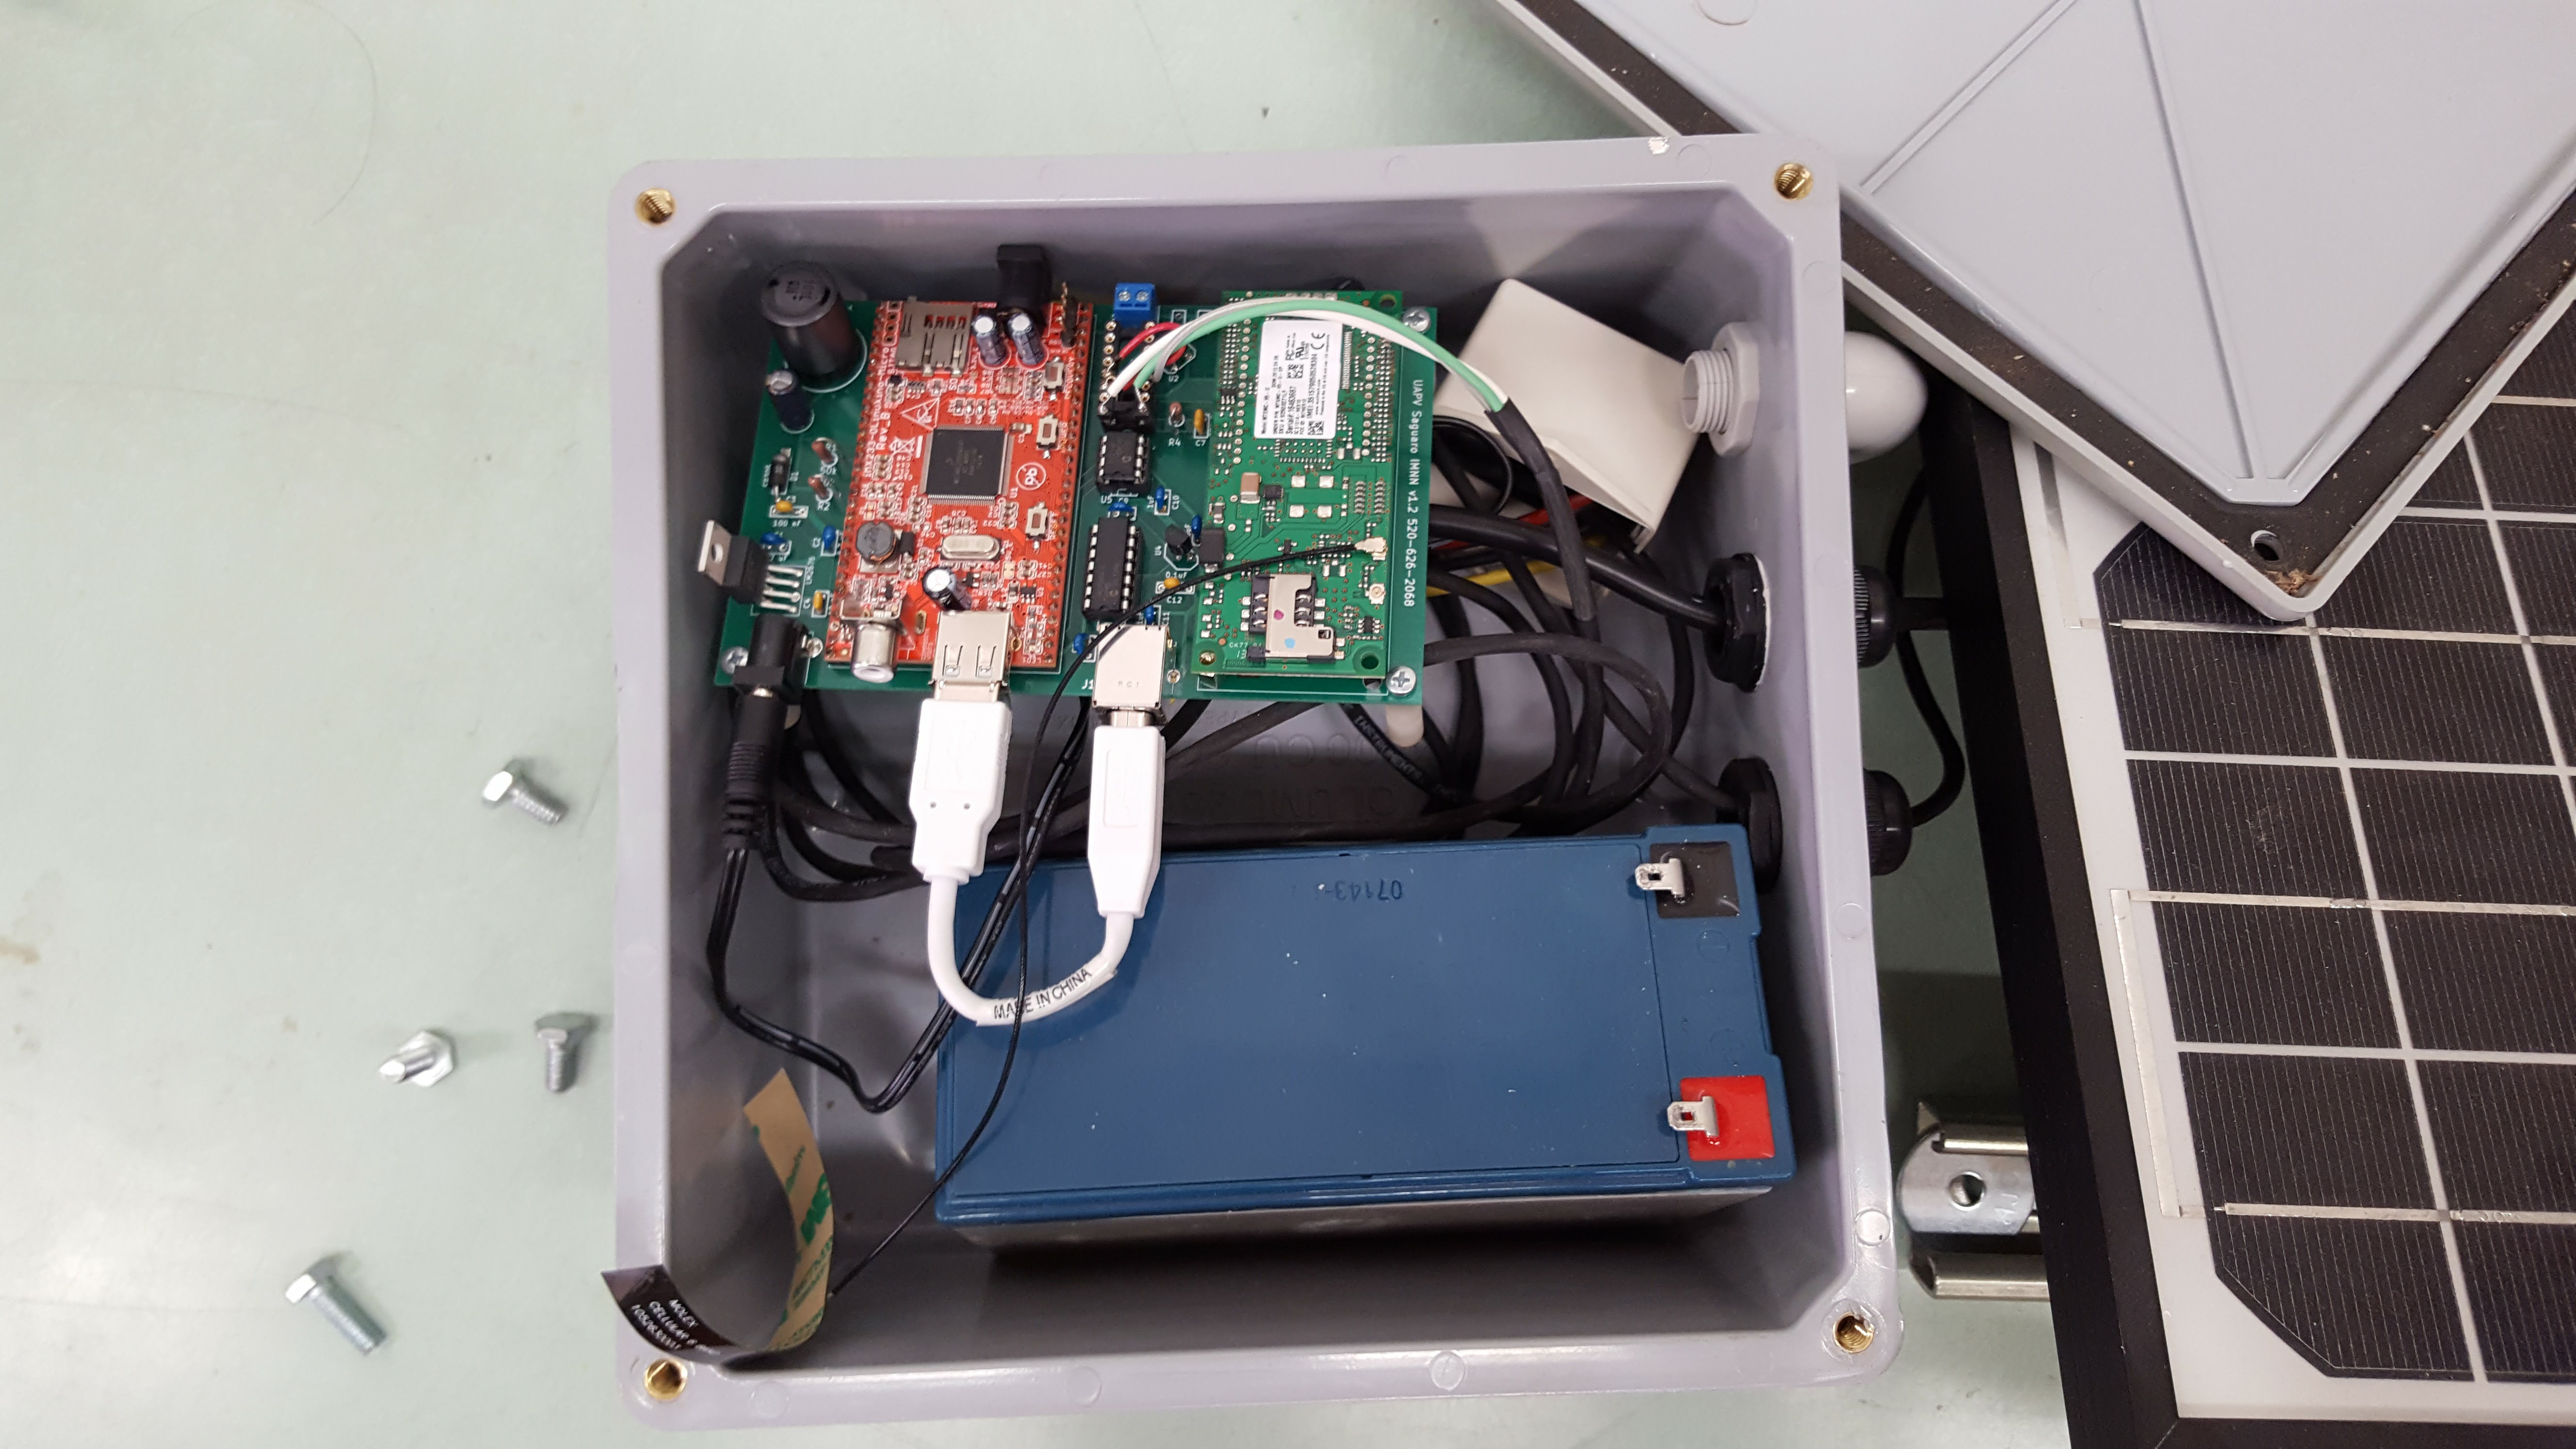
\includegraphics[width=\textwidth]{../dissertation/figs/sensor_interior.jpg}
\end{figure}
\end{column}
\begin{column}{0.2\textwidth}
\begin{figure}[h]
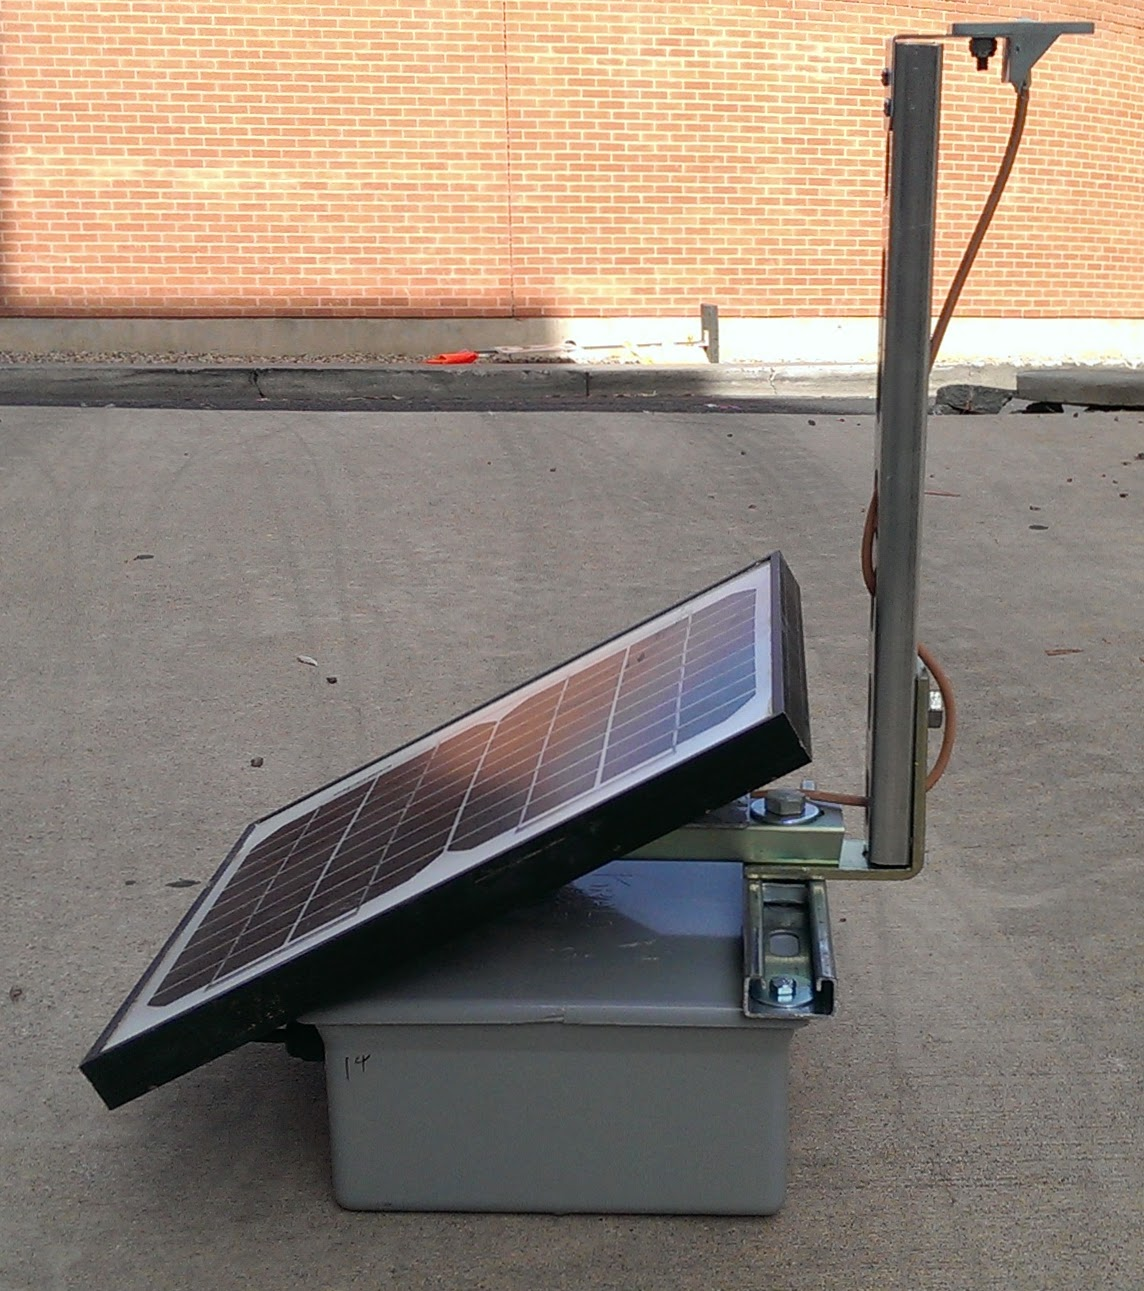
\includegraphics[height=.5\textheight]{../dissertation/figs/sensor_outside.jpg}
\end{figure}
\end{column}
\begin{column}{0.4\textwidth}
\begin{figure}[h]
\centering
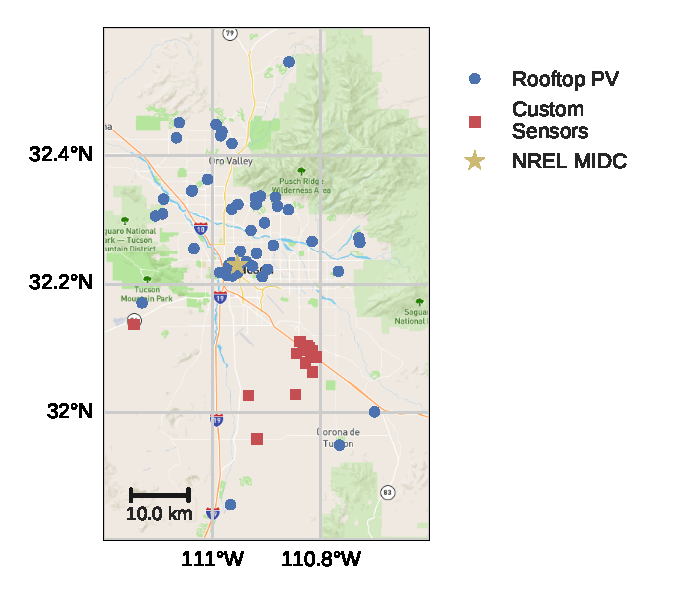
\includegraphics[height=0.7\textheight]{../dissertation/figs/map.pdf}
\end{figure}
\end{column}
\end{columns}
\end{frame}

\section{Irradiance Network Forecasts}
\begin{frame}{Irradiance Network Forecasts}
\begin{figure}[h]
  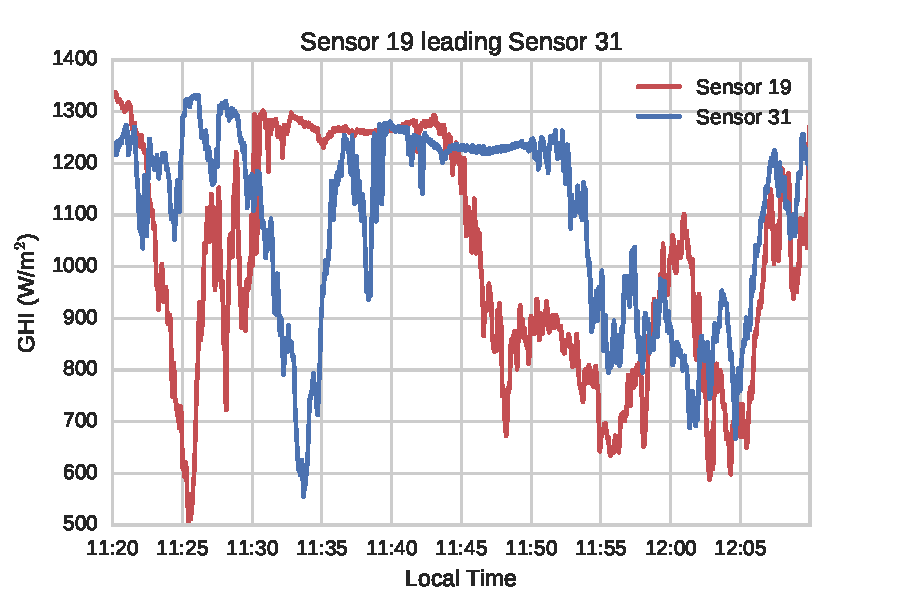
\includegraphics[height=.8\textheight]{../dissertation/figs/leading_sens.pdf}
\end{figure}
\end{frame}

\begin{frame}{Irradiance Network Forecasts}
\begin{figure}[h]
  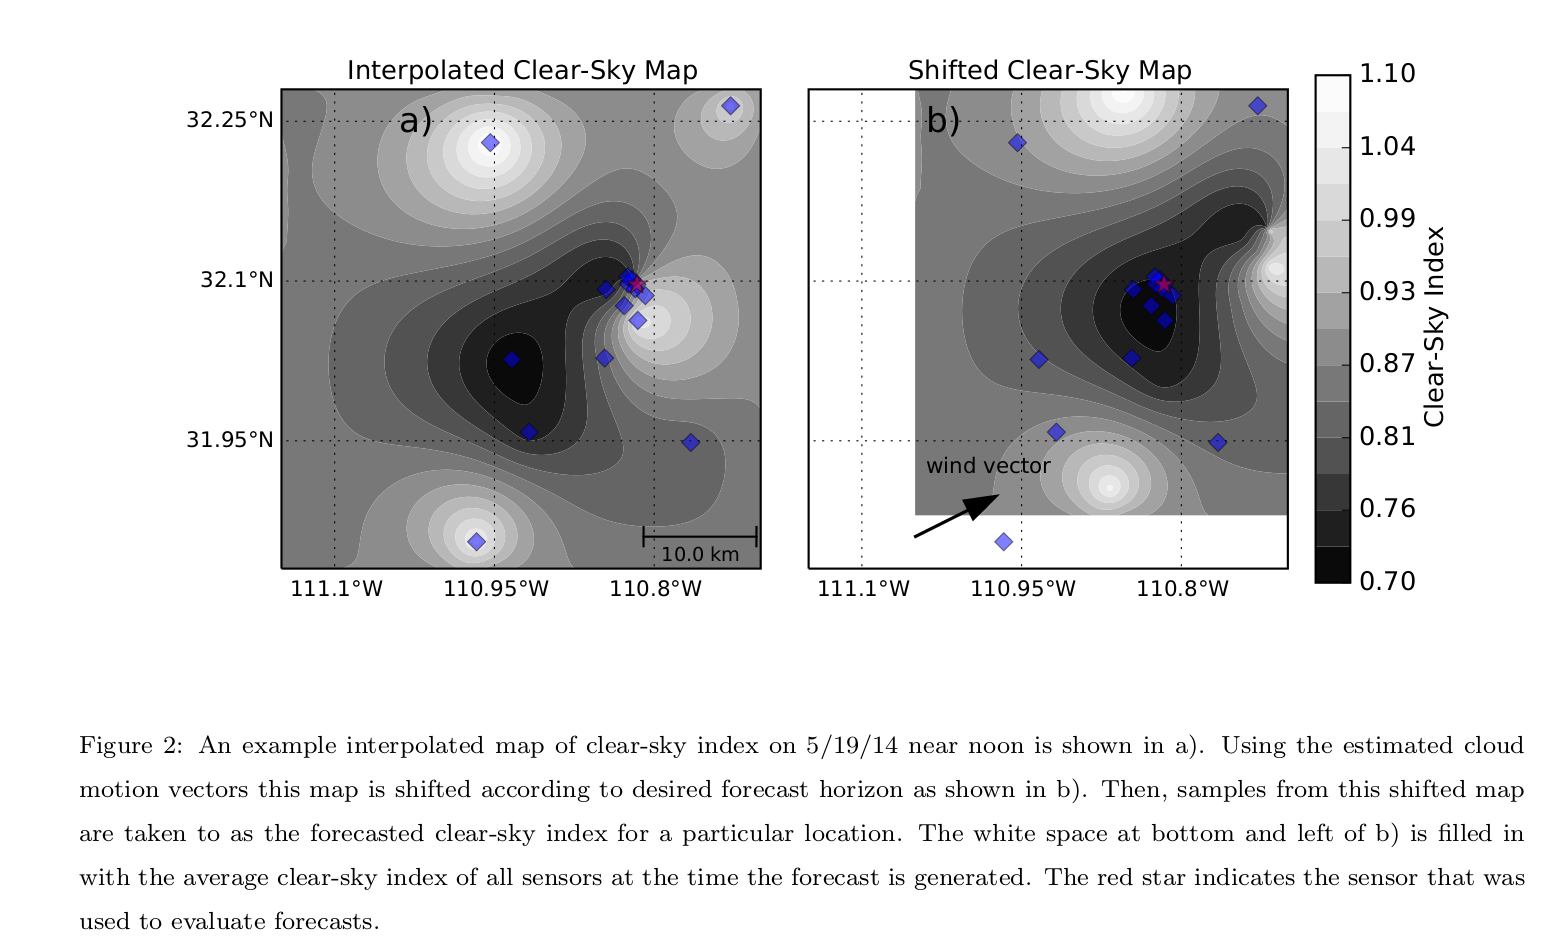
\includegraphics[height=0.8\textheight]{figs/interpmap.png}
\end{figure}
\end{frame}

\begin{frame}{Forecast Error Metrics}
\begin{columns}
\begin{column}{0.4\textwidth}
\begin{figure}[h]
  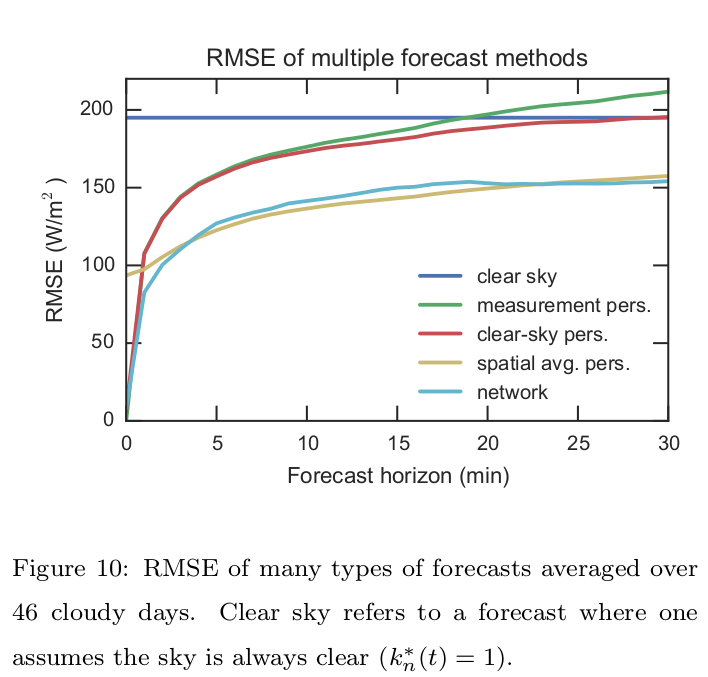
\includegraphics[width=\textwidth]{figs/network_rmse.png}
\end{figure}
\end{column}
\begin{column}{0.3\textwidth}
\begin{figure}[h]
  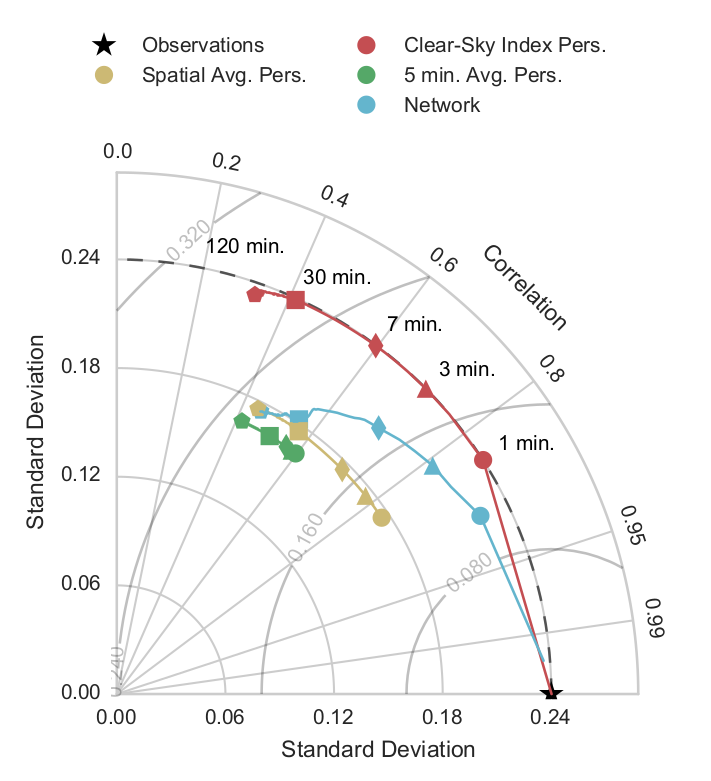
\includegraphics[height=.7\textheight]{figs/old_taylor.png}
\end{figure}
\end{column}
\begin{column}{0.3\textwidth}
\begin{figure}[h]
  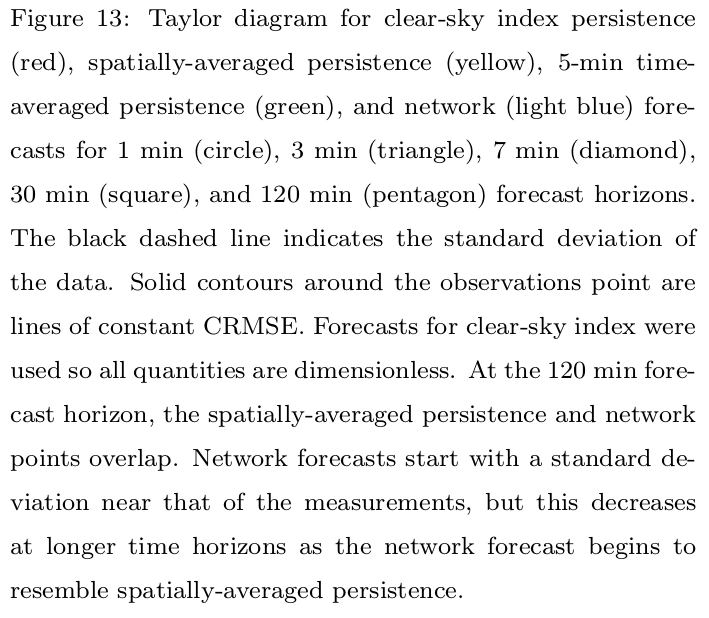
\includegraphics[height=.5\textheight]{figs/old_taylor_cap.png}
\end{figure}
\end{column}
\end{columns}
\end{frame}

\section[Optimal Interpolation]{Optimal Interpolation of Satellite
  Derived Irradiance and Network Data}
\begin{frame}{Optimal Interpolation}
\begin{columns}
\begin{column}{0.4\textwidth}
\begin{figure}[h]
  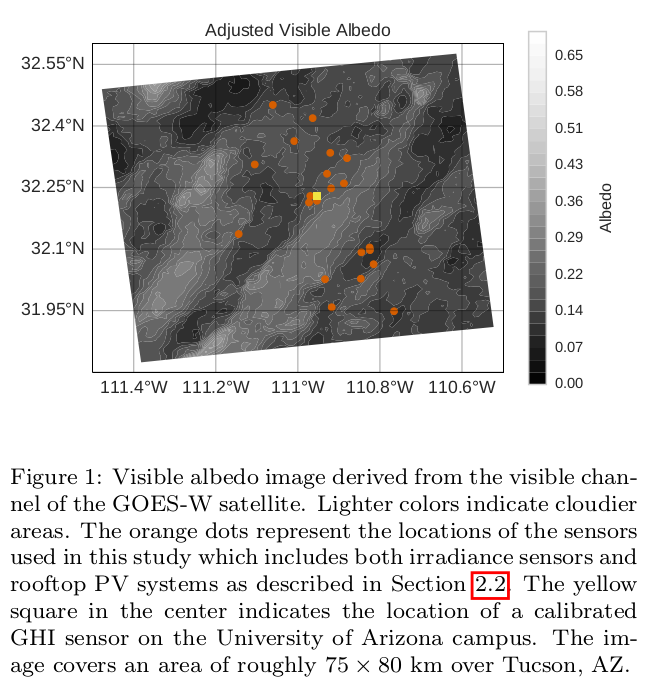
\includegraphics[height=.7\textheight]{figs/satimg.png}
\end{figure}
\end{column}
\begin{column}{0.6\textwidth}
\begin{figure}[h]
  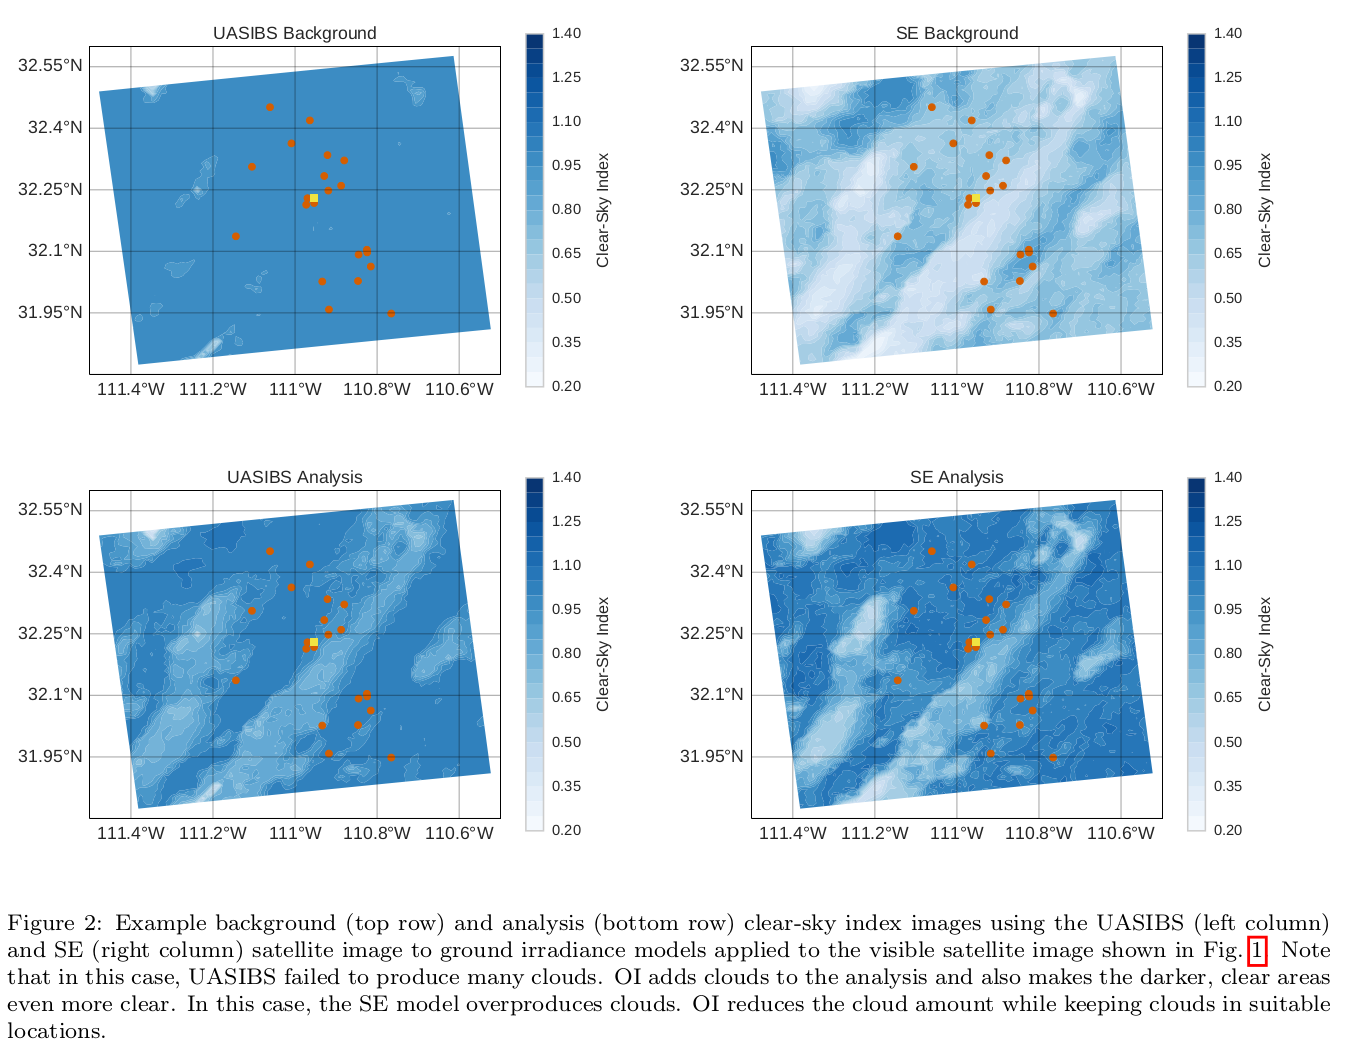
\includegraphics[height=.7\textheight]{figs/satoi_improv.png}
\end{figure}
\end{column}
\end{columns}
\end{frame}

\begin{frame}{OI Corrections}
\begin{figure}[h]
  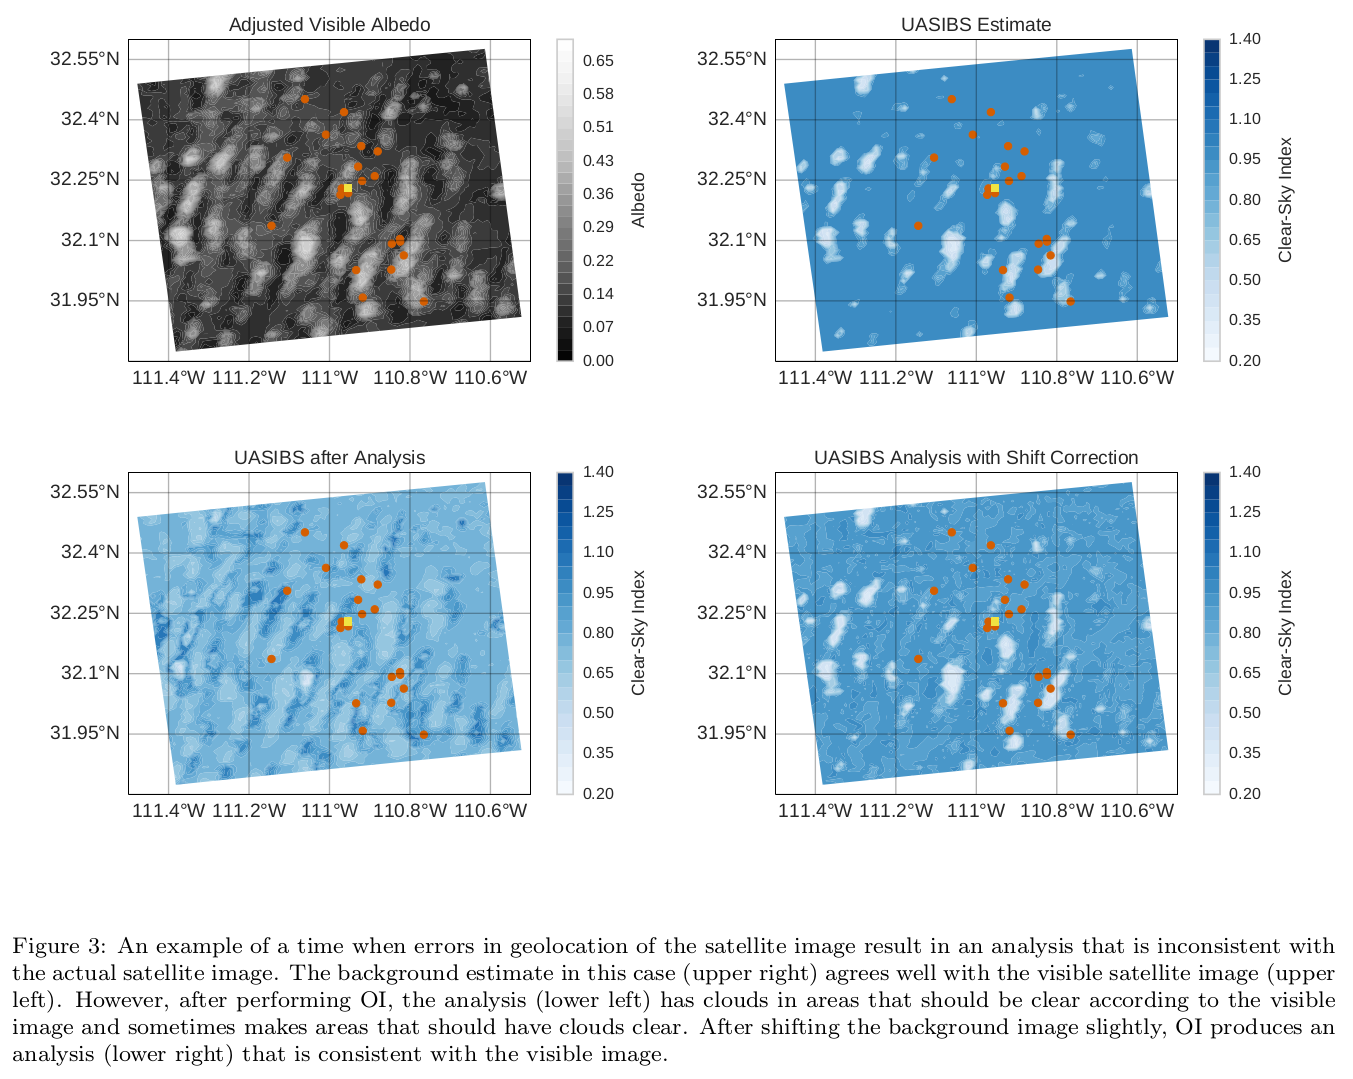
\includegraphics[height=.7\textheight]{figs/parallax.png}
\end{figure}
\end{frame}

\section{Conclusion}
\begin{frame}{Conclusion}
\begin{figure}[h]
  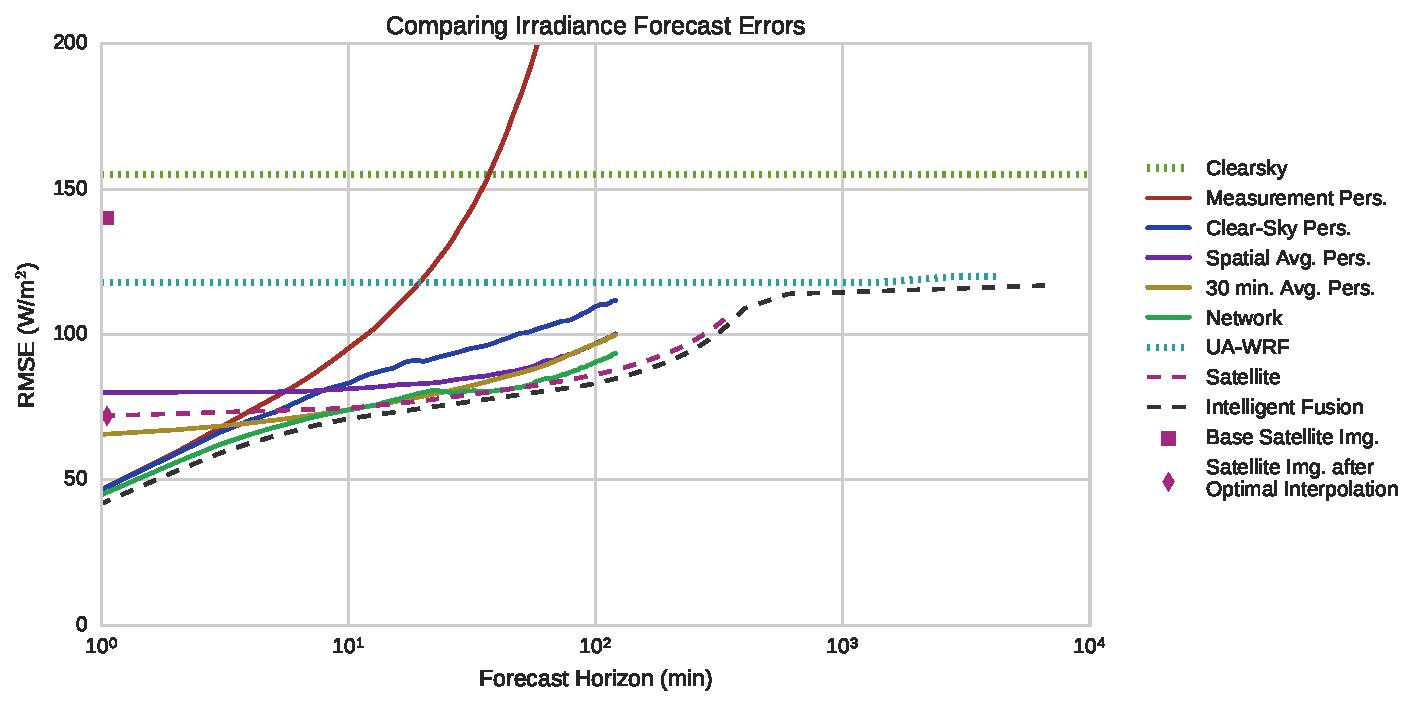
\includegraphics[width=.8\textwidth]{../dissertation/figs/timehorizon.pdf}
\end{figure}
\end{frame}

\begin{frame}{Publications}
\fontsize{8}{12}
\begin{itemize}
  \item  A. T. Lorenzo, W. F. Holmgren, M. Leuthold, C. K. Kim,
  A. D. Cronin, and E. a. Betterton, ``Short-term PV power forecasts
  based on a real-time irradiance monitoring network,'' in 2014 IEEE
  40th Photovoltaic Specialist Conference (PVSC), 2014, pp. 0075-–0079.
\item A. T. Lorenzo, W. F. Holmgren, and A. D. Cronin, ``Irradiance
  forecasts based on an irradiance monitoring network, cloud motion,
  and spatial averaging,'' Sol. Energy, vol. 122, pp. 1158-–1169, 2015.
\item A. T. Lorenzo, M. Morzfeld, W. F. Holmgren, and A. D. Cronin,
  ``Optimal Interpolation of Satellite Derived Irradiance and Ground
  Data,'' in 2016 IEEE 43th Photovoltaic Specialist Conference (PVSC),
  2016.
\item A. T. Lorenzo, M. Morzfeld, W. F. Holmgren, and A. D. Cronin, ``Optimal interpolation of satellite and ground data for irradiance nowcasting at city scales,'' Sol. Energy, vol. 144, pp. 466-–474, 2017.
\end{itemize}
\end{frame}

\begin{frame}{Presentations \& Posters}
\fontsize{8}{12}
\begin{columns}
\begin{column}{0.5 \textwidth}
Presentations
\begin{itemize}
  \item  PVSC 2014, ``Short-term PV power forecasts
  based on a real-time irradiance monitoring network''
\item AZSEC 2015, ``Operational Wind and Solar Power Forecasting in
  the Southwest''
\item PVSC 2016, ``Optimal Interpolation of Satellite Derived Irradiance and Ground
  Data''
\end{itemize}
\end{column}
\begin{column}{0.5\textwidth}
Posters
\begin{itemize}
\item AMS 2015, ``Intra-hour solar power forecasts using a real-time
  irradiance monitoring network''
\item AGU 2016, ``Fusing Satellite-Derived Irradiance and Point
  Measurements through Optimal Interpolation''
\item AMS 2017, ``nabu: A distributed, parallel, data processing platform''
\end{itemize}
\end{column}
\end{columns}
\end{frame}

\begin{frame}{Classes}
\fontsize{8}{12}
\begin{columns}
\begin{column}{0.5 \textwidth}
\begin{itemize}
\item OPTI 501 Electromagnetic Waves
\item OPTI 502 Optical Design and Instrumentation
\item OPTI 506 Radiometry, Sources \& Detectors
\item OPTI 507 Solid State Optics
\item OPTI 508 Probability \& Statistical Optics
\item OPTI 510R Photonics
\item OPTI 511L Laser \& Solid State Lab
\item OPTI 512L Mathematical Optics Lab
\item OPTI 514A Photovoltaic Solar Energy Systems
\item OPTI 544 Foundations of Quantum Optics
\end{itemize}
\end{column}
\begin{column}{0.5 \textwidth}
\begin{itemize}
\item OPTI 546 Physical Optics
\item OPTI 570A Quantum Mechanics
\item OPTI 637 Principles of Image Science
\item ATMO 536A Fundamentals of Atmospheric Sciences
\item ATMO 545 Intro to Data Assimilation
\item ATMO 558 Mesoscale Meteorological Modeling
\item MATH 599 Independent Study
\item OPTI 589 Optics Outreach
\item LIBR 696A Info Research Strategies
\end{itemize}
\end{column}
\end{columns}
\end{frame}

\end{document}

%%% Local Variables:
%%% mode: latex
%%% TeX-master: t
%%% End:
